\documentclass[12pt]{article}

\usepackage{sbc-template}
\usepackage{graphicx,url}
\usepackage{placeins}
\usepackage{multirow}
\usepackage[utf8]{inputenc}
\usepackage[brazil]{babel}
%\usepackage[latin1]{inputenc}  

     
\sloppy

\title{Predição de Satisfação de Passageiros em Aeroportos Brasileiros: Uma Abordagem com LightGBM e SHAP Values}

\author{Helio José\inst{1}, Ludson Lira\inst{1}, Raul Alves\inst{1}, Walber Luis\inst{1}, Kaue Patricius\inst{1}}


\address{Instituto de Computação -- Universidade Federal de Alagoas (UFAL)\\
  Maceió -- AL -- Brazil
  \email{\{helio, ludson, raul, walber, kaue\}@ic.ufal.br}
}

\begin{document} 

\maketitle

\begin{abstract}
  This paper addresses the problem of predicting passenger satisfaction in Brazilian airports. Passenger experience is a critical metric for evaluating airport management quality, yet identifying its key drivers remains challenging. We applied Machine Learning techniques on real data from the National Civil Aviation Secretariat to build a predictive model. Using the LightGBM algorithm, the proposed model achieved an accuracy of 81.72\% and an AUC-ROC of 0.8957.
\end{abstract}
     
\begin{resumo} 
  Este artigo aborda o problema de prever a satisfação dos passageiros em aeroportos brasileiros. A experiência do passageiro é uma métrica crítica para avaliar a qualidade da gestão aeroportuária, porém identificar seus principais determinantes é um desafio. Aplicamos técnicas de Aprendizado de Máquina em dados reais da Secretaria Nacional de Aviação Civil para construir um modelo preditivo. Utilizando o algoritmo LightGBM, o modelo proposto alcançou uma acurácia de 81,72\% e um AUC-ROC de 0,8957.
\end{resumo}


\section{Introdução}

A experiência do passageiro tornou-se um fator estratégico vital para companhias aéreas e administradores aeroportuários no século XXI. Em um setor altamente competitivo e globalizado, a qualidade dos serviços prestados em terra, desde o momento do check-in até a restituição de bagagens no desembarque, é determinante para a fidelização do cliente e para a imagem institucional das empresas envolvidas. Historicamente, a gestão da satisfação era conduzida de forma reativa, baseando-se majoritariamente em reclamações formais e ouvidorias. No entanto, o paradigma atual exige abordagens proativas, onde intervenções operacionais são antecipadas através de padrões detectados em grandes volumes de dados.

No cenário brasileiro, observa-se uma lacuna significativa: apesar da abundância de dados coletados, há uma escassez de modelos preditivos consolidados que utilizem dados reais e em larga escala de aeroportos nacionais para inferência direta. A Secretaria Nacional de Aviação Civil (SNAC) conduz pesquisas regulares de satisfação, mas o potencial analítico dessas informações é frequentemente subutilizado em relatórios meramente descritivos. Tais relatórios falham em capturar as interações não lineares entre variáveis complexas, como o impacto cruzado entre o tempo de espera na segurança e o conforto térmico da sala de embarque.

Para preencher essa lacuna, este trabalho apresenta um pipeline completo de Aprendizado de Máquina focado em prever a satisfação de passageiros. Utilizamos um conjunto de dados públicos contendo 57.514 registros reais e 145 variáveis oriundas da SNAC, abrangendo o período de maior movimentação dos principais terminais brasileiros. O processo engloba desde um tratamento robusto de dados (lidando com mais de 3 milhões de nulos) até a comparação empírica de cinco algoritmos de última geração, culminando na adoção de métodos de explicabilidade (SHAP) para a extração de inteligência operacional.

As principais contribuições deste estudo são: (i) a validação empírica de hipóteses de negócio sobre a satisfação em aeroportos brasileiros, revelando que fatores operacionais de base superam atrativos comerciais em peso de decisão; (ii) a proposição de um modelo preditivo baseado no algoritmo LightGBM que atinge um AUC-ROC de 0.8957, demonstrando alta capacidade de discriminação; e (iii) a análise de explicabilidade via valores SHAP, que transforma o modelo matemático em um roteiro de recomendações diretamente acionáveis para gestores e concessionárias aeroportuárias.

O restante deste artigo está organizado da seguinte forma: a Seção 2 apresenta os trabalhos relacionados e o estado da arte. A Seção 3 descreve detalhadamente a base de dados e os processos de pré-processamento. A Seção 4 detalha a metodologia de construção da "Arena de Algoritmos" e as estratégias de validação. A Seção 5 expõe e discute os resultados dos experimentos e a análise de explicabilidade. A Seção 6 traz a discussão sobre o impacto prático e as implicações táticas dos achados. Por fim, a Seção 7 encerra o trabalho com as conclusões e as perspectivas para investigações futuras.

\section{Trabalhos Relacionados}

A avaliação da qualidade de serviços em transportes tem raízes no modelo SERVQUAL, proposto por Parasuraman, Zeithaml e Berry \cite{parasuraman1988servqual}, que estrutura a percepção do consumidor em cinco dimensões (tangibilidade, confiabilidade, responsividade, garantia e empatia). Essa abordagem influenciou fortemente a pesquisa em aviação, onde métricas como o \textit{Net Promoter Score} (NPS), introduzido por Reichheld \cite{reichheld2003nps}, passaram a ser amplamente adotadas como indicadores de fidelização. Entretanto, tanto o SERVQUAL quanto o NPS capturam apenas relações lineares e agregadas, limitando a compreensão granular dos motivadores específicos de insatisfação em contextos de alta dimensionalidade.

Com a evolução computacional, o foco deslocou-se para abordagens de Aprendizado de Máquina. Noviantoro e Huang \cite{noviantoro2022investigating}, em estudo publicado na \textit{Research in Transportation Business \& Management}, aplicaram técnicas de mineração de dados ao problema de satisfação de passageiros aéreos, demonstrando que modelos de \textit{ensemble} superam significativamente modelos lineares ao capturar interações complexas entre atributos categóricos e numéricos. Nesse contexto, algoritmos de \textit{gradient boosting} como o XGBoost \cite{chen2016xgboost} e o LightGBM \cite{ke2017lightgbm} vêm se consolidando como referências para dados tabulares de alta dimensionalidade, oferecendo uma combinação favorável de acurácia, robustez a ruídos e eficiência computacional.

Paralelamente, a necessidade de inteligência acionável motivou a incorporação de técnicas de explicabilidade (\textit{eXplainable AI} - XAI). O desafio de modelos complexos reside em sua natureza de "caixa-preta", o que dificulta a confiança de gestores em decisões críticas. Os valores SHAP (\textit{SHapley Additive exPlanations}), baseados na teoria dos jogos cooperativos introduzida por Lundberg e Lee \cite{lundberg2017}, tornaram-se o padrão-ouro para essa finalidade. Eles permitem desmembrar a contribuição de cada variável (como "limpeza" ou "tempo de fila") no veredito final do modelo, oferecendo consistência tanto a nível individual quanto global.

Diferente dos trabalhos supracitados, que se apoiam em bases de dados internacionais ou restritas a uma única companhia aérea, este estudo utiliza dados abertos do governo federal brasileiro \cite{snac_dados}, abrangendo múltiplos aeroportos e concessionárias sob a regulação da ANAC/SNAC. Isso confere ao trabalho uma validade externa superior para o contexto nacional. A Tabela~\ref{tab:related_works} consolida o posicionamento deste estudo frente às abordagens identificadas na literatura.

\begin{table}[ht]
\centering
\caption{Comparação com a Literatura}
\label{tab:related_works}
\resizebox{\textwidth}{!}{
\begin{tabular}{|l|l|l|l|}
\hline
\textbf{Trabalho} & \textbf{Dataset} & \textbf{Método Principal} & \textbf{Métrica de Destaque} \\
\hline
Parasuraman et al. \cite{parasuraman1988servqual} & Questionários multissetoriais & SERVQUAL (escala) & Gaps de qualidade \\
Noviantoro e Huang \cite{noviantoro2022investigating} & Airline Satisfaction (internacional) & Data Mining, Random Forest & Acurácia \\
\textbf{Nossa Abordagem} & \textbf{SNAC Brasil (57.5k registros)} & \textbf{LightGBM + SHAP} & \textbf{AUC-ROC (0.8957)} \\
\hline
\end{tabular}
}
\end{table}

\section{Base de Dados e Pré-processamento}

\subsection{Origem e Caracterização}
Os dados utilizados neste estudo foram extraídos dos Dados Abertos da Secretaria Nacional de Aviação Civil \cite{snac_dados}, os quais contêm os resultados da Pesquisa de Satisfação do Passageiro realizada trimestralmente em diversos aeroportos do Brasil. A base original engloba 57.514 registros e 145 variáveis, retratando uma rica complexidade de informações operacionais, demográficas e de percepção de serviço. As variáveis cobrem desde o tempo de antecedência da chegada ao aeroporto até avaliações detalhadas de 1 a 5 para quesitos como limpeza, sinalização, cordialidade dos funcionários e qualidade do Wi-Fi. A variável alvo, denominada \texttt{liked}, é uma derivação binária da percepção geral, apresentando uma distribuição equilibrada (aproximadamente 50/50 entre satisfeitos e insatisfeitos). Esse equilíbrio natural é uma característica valiosa do \textit{dataset}, pois elimina a necessidade de técnicas sintéticas de balanceamento, como o SMOTE \cite{chawla2002smote}, que poderiam introduzir ruídos no modelo.

\subsection{Desafios e Tratamento de Nulos}
A etapa de pré-processamento exigiu um tratamento rigoroso e semanticamente consciente, pois o \textit{dataset} bruto possuía mais de 3,3 milhões de valores nulos (3.323.783, especificamente). A estratégia adotada foi dividida em duas frentes complementares:
\begin{itemize}
    \item \textbf{Tratamento Estrutural}: Avaliou-se o uso de \textit{flags} de aplicabilidade (\texttt{\_is\_applicable}). Muitos nulos na base não indicam falta de informação, mas sim a não ocorrência do serviço para aquele perfil de passageiro (ex: um passageiro em voo doméstico não passa pela imigração ou controle alfandegário). Nesses casos, a nota nula foi imputada estruturalmente como $-1$, permitindo que o modelo aprenda que a ausência do serviço é um estado válido e distinto de uma nota baixa.
    \item \textbf{Imputação de Resíduos}: Para os valores nulos remanescentes que não possuíam justificativa estrutural, utilizou-se a imputação estatística clássica: preenchimento pela mediana nas variáveis numéricas (para mitigar o impacto de \textit{outliers}) e pela moda nas variáveis categóricas.
\end{itemize}

\subsection{Engenharia de Atributos e Codificação}
Após o tratamento de nulos, as 23 variáveis categóricas remanescentes (como aeroporto de origem, destino e companhia aérea) foram submetidas à técnica de \textit{One-Hot Encoding}. Esse procedimento expandiu o espaço amostral de atributos, resultando em um \textit{dataset} final robusto com 252 variáveis independentes. Adicionalmente, realizou-se a normalização dos nomes das colunas, removendo caracteres especiais e espaços para garantir compatibilidade estrutural estrita com os algoritmos de \textit{Gradient Boosting}, como o LightGBM. A Figura~\ref{fig:pipeline} ilustra o fluxograma desse processo, evidenciando a transformação dos dados brutos em uma matriz numérica de alta fidelidade.

\begin{figure}[ht]
\centering
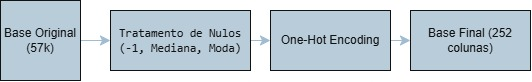
\includegraphics[width=0.6\textwidth]{fig1.jpg}
\caption{Fluxograma do pipeline de dados, desde a extração até o modelo treinado.}
\label{fig:pipeline}
\end{figure}

\begin{table}[ht]
\centering
\caption{Estatísticas Descritivas e Tratamento de Dados}
\label{tab:descritiva}
\begin{tabular}{|l|c|c|}
\hline
\textbf{Característica} & \textbf{Valor Original} & \textbf{Após Tratamento} \\
\hline
Total de Registros & 57.514 & 57.514 \\
Total de Variáveis & 145 & 252 \\
Valores Nulos & 3.323.783 & 0 \\
Técnica Categórica & Textos brutos & One-Hot Encoding \\
\hline
\end{tabular}
\end{table}

\section{Metodologia}

Para avaliar as hipóteses de negócio e predizer a satisfação de passageiros, foi elaborada uma "Arena de Algoritmos". Esta abordagem consiste em testar sistematicamente modelos de complexidade crescente sob as mesmas condições amostrais, permitindo uma escolha fundamentada pelo princípio da parcimônia e pela performance estatística.

\subsection{Algoritmos Avaliados}
Cinco abordagens de aprendizado supervisionado foram selecionadas para a competição:
\begin{enumerate}
    \item \textbf{Regressão Logística}: Implementada com \textit{solver} 'lbfgs' e 1000 iterações, servindo como o \textit{baseline} estatístico para capturar relações lineares simples.
    \item \textbf{Árvore de Decisão}: Configurada com profundidade máxima de 8 para evitar \textit{overfitting} inicial e fornecer uma base de regras de decisão clara.
    \item \textbf{Random Forest} \cite{breiman2001random}: Utilizando 100 estimadores, focando na redução de variância através do \textit{bagging} e captura de interações não lineares complexas.
    \item \textbf{XGBoost} \cite{chen2016xgboost}: Uma implementação de \textit{gradient boosting} de alta performance, configurada com \textit{learning rate} de 0.1 e profundidade 6.
    \item \textbf{LightGBM} \cite{ke2017lightgbm}: Escolhido como o candidato principal devido à sua eficiência nativa no tratamento de alta dimensionalidade (comum após \textit{encoding}) e sua rapidez no processamento de grandes volumes de dados.
\end{enumerate}

\subsection{Estratégia de Validação e Métricas}
A validação técnica seguiu o formato \textit{Hold-out}, segregando a base em 80\% para treinamento (46.011 amostras) e 20\% para testes isolados (11.503 amostras). Utilizou-se estratificação em relação à variável alvo para assegurar que a proporção 50/50 fosse rigorosamente preservada em todos os subconjuntos.

Adicionalmente, empregou-se a Validação Cruzada K-Fold ($K=5$) no conjunto de treinamento. Este procedimento divide os dados de treino em 5 fatias, treinando e validando o modelo 5 vezes, alternando a fatia de validação. Isso garante que as métricas reportadas não sejam fruto de uma divisão "afortunada" dos dados, mitigando vieses de sobreajuste. A principal métrica estabelecida foi a Área Sob a Curva ROC (AUC-ROC), por melhor representar a capacidade de discriminação do modelo ao avaliar custos de erros de classificação. Também analisou-se acurácia, \textit{precision}, \textit{recall} e F1-Score para uma visão holística da performance.

\subsection{Explicabilidade com SHAP}
Para romper com a natureza de "caixa-preta" dos modelos de \textit{boosting}, integrou-se a técnica SHAP. Baseada na teoria dos jogos cooperativos, a técnica calcula o valor de Shapley para cada variável, garantindo uma distribuição justa do ganho de informação. Matematicamente, a contribuição $\phi_i$ de um atributo $i$ para a predição do modelo $f$ sobre uma amostra $x$ é dada por:

\begin{equation}
\phi_i(f, x) = \sum_{S \subseteq F \setminus \{i\}} \frac{|S|! (|F| - |S| - 1)!}{|F|!} [f_x(S \cup \{i\}) - f_x(S)]
\end{equation}

Onde $F$ representa o conjunto de todas as \textit{features} e $S$ um subconjunto sem a \textit{feature} $i$. Essa formulação permite isolar a contribuição marginal de atributos como "limpeza" ou "infraestrutura", desmembrando como cada variável empurra o veredito do modelo em direção ao polo promotor ou detrator. Diferentemente das importâncias tradicionais baseadas em ganho de entropia, o SHAP oferece consistência local e global. Essa etapa matemática é crucial para transformar a performance preditiva bruta em recomendações de negócio sólidas e diretamente acionáveis pelos gestores aeroportuários.
\section{Experimentos e Resultados}

\subsection{Análise Descritiva da Base e Comportamento das Variáveis}
A avaliação exploratória inicial confirmou que a variável alvo \texttt{liked} apresenta uma distribuição notavelmente balanceada. Este equilíbrio natural na base de dados é fundamental, pois elimina potenciais vieses de classe na predição e descarta a necessidade de aplicar técnicas sintéticas de balanceamento e reamostragem, como o SMOTE (\textit{Synthetic Minority Over-sampling Technique}) \cite{chawla2002smote}, que poderiam introduzir ruídos indesejados. A Figura~\ref{fig:distribuicao} ilustra essa distribuição, assegurando que o algoritmo terá instâncias suficientes de ambas as classes para extrair padrões robustos.

\begin{figure}[ht]
\centering
\includegraphics[width=0.5\textwidth]{fig2.png}
\caption{Distribuição da variável alvo (\texttt{liked}), demonstrando o balanceamento natural da base.}
\label{fig:distribuicao}
\end{figure}

Além da distribuição da classe alvo, a análise de associação de variáveis foi conduzida através de uma matriz de correlação. Avaliando a matriz (Figura~\ref{fig:heatmap}), notou-se que atributos operacionais básicos, como \textit{Location and Movement} e \textit{Limpeza Geral}, são os que mais covariam positivamente com a nota final de satisfação. Esse achado sugere uma forte relação linear preliminar entre o bem-estar físico do passageiro no terminal e a sua percepção final do serviço prestado. Por outro lado, serviços acessórios e opções comerciais apresentaram correlações significativamente menores, indicando que investimentos nesses setores podem ter um impacto apenas marginal na satisfação global quando comparados à infraestrutura de base.

\begin{figure}[ht]
\centering
\includegraphics[width=0.7\textwidth]{fig3.png}
\caption{Matriz de Correlação das principais variáveis (Top 15 + Liked) destacando o impacto linear na satisfação.}
\label{fig:heatmap}
\end{figure}

\subsection{Performance Comparativa dos Modelos e Validação Cruzada}
Os resultados obtidos na etapa que denominamos "Arena de Algoritmos" demonstraram uma superioridade empírica clara e incontestável dos métodos baseados em árvores e, mais especificamente, em \textit{gradient boosting}. A Tabela~\ref{tab:cv_results} detalha as acurácias médias obtidas via validação cruzada ($K=5$) para cada modelo testado, evidenciando a evolução do poder preditivo conforme a complexidade do modelo aumenta.

\begin{table}[ht]
\centering
\caption{Resultados da Arena de Algoritmos (Acurácia Média CV)}
\label{tab:cv_results}
\begin{tabular}{|l|c|c|}
\hline
\textbf{Algoritmo} & \textbf{Acurácia Média} & \textbf{Desvio Padrão ($\pm$)} \\
\hline
Regressão Logística & 79,71\% & 0,59\% \\
Árvore de Decisão & 79,30\% & 0,92\% \\
Random Forest & 80,24\% & 0,48\% \\
XGBoost & 81,61\% & 0,74\% \\
\textbf{LightGBM} & \textbf{81,72\%} & \textbf{0,66\%} \\
\hline
\end{tabular}
\end{table}

A Regressão Logística, utilizada como \textit{baseline}, apresentou um desempenho surpreendentemente robusto, indicando que uma parcela significativa da satisfação pode ser explicada por relações lineares simples. Entretanto, o modelo enfrentou dificuldades para capturar as interações complexas entre variáveis como aeroporto de origem e tipo de voo. As Árvores de Decisão, embora intuitivas, sofreram com instabilidade e uma leve tendência ao \textit{overfitting}, apresentando o maior desvio padrão entre os modelos testados.

O Random Forest mitigou parte dessa instabilidade através do \textit{bagging}, mas foram os algoritmos de \textit{Gradient Boosting} (XGBoost e LightGBM) que atingiram o patamar de $81\%$. O \textbf{LightGBM} sagrou-se o modelo vencedor, atingindo uma acurácia de $81,72\%$. Ao ser avaliado no conjunto de teste isolado ($hold-out$), o modelo manteve sua performance com uma acurácia de $82\%$ e um valor de Área Sob a Curva ROC (AUC-ROC) de $0,8957$. Essa métrica consolida a excelente capacidade do algoritmo em generalizar padrões complexos e garantir uma separabilidade eficaz entre as classes. A Tabela~\ref{tab:classification_report} apresenta o relatório de classificação detalhado para o modelo campeão, demonstrando um equilíbrio saudável entre \textit{precision} e \textit{recall} para ambas as classes.

\begin{table}[ht]
\centering
\caption{Relatório de Classificação (LightGBM)}
\label{tab:classification_report}
\begin{tabular}{|l|c|c|c|c|}
\hline
\textbf{Classe} & \textbf{Precision} & \textbf{Recall} & \textbf{F1-Score} & \textbf{Suporte} \\
\hline
0 (Insatisfeito) & 0,85 & 0,77 & 0,81 & 5.752 \\
1 (Satisfeito) & 0,79 & 0,86 & 0,82 & 5.751 \\
\hline
\textbf{Acurácia} & \multicolumn{3}{c|}{\textbf{0,82}} & \textbf{11.503} \\
\hline
\end{tabular}
\end{table}

Para complementar a avaliação de \textit{Precision} e \textit{Recall}, a análise de erros foi aprofundada por meio da Matriz de Confusão do modelo vencedor (Tabela~\ref{tab:confusion_matrix}). A partir dos 11.503 passageiros avaliados no conjunto de teste, o modelo foi capaz de acertar corretamente 4.429 instâncias de passageiros insatisfeitos (Verdadeiros Negativos) e 4.946 instâncias de passageiros satisfeitos (Verdadeiros Positivos). 

\begin{table}[ht]
\centering
\caption{Matriz de Confusão do LightGBM no Conjunto de Teste}
\label{tab:confusion_matrix}
\begin{tabular}{|l|c|c|c|}
\hline
\multicolumn{2}{|c|}{} & \multicolumn{2}{c|}{\textbf{Classe Predita}} \\
\cline{3-4}
\multicolumn{2}{|c|}{} & \textbf{Insatisfeito (0)} & \textbf{Satisfeito (1)} \\
\hline
\multirow{2}{*}{\textbf{Classe Real}} & \textbf{Insatisfeito (0)} & 4.429 (VN) & 1.323 (FP) \\
\cline{2-4}
& \textbf{Satisfeito (1)} & 805 (FN) & 4.946 (VP) \\
\hline
\end{tabular}
\end{table}

A distribuição de erros revela um aspecto importante sobre os custos de classificação no contexto de negócios. O modelo gerou 1.323 Falsos Positivos (Erro Tipo I), ou seja, casos em que o sistema previu que o passageiro estava satisfeito, quando na verdade ele era um detrator. Estrategicamente, este é o erro mais perigoso para as concessionárias, pois mascara usuários insatisfeitos que poderiam registrar queixas formais. Por outro lado, registraram-se apenas 805 Falsos Negativos (Erro Tipo II), o que indica que o modelo é razoavelmente conservador e tende a errar menos ao classificar alguém erroneamente como insatisfeito. Em um cenário real, um Falso Negativo resultaria em um pedido de \textit{feedback} adicional ou em uma abordagem preventiva desnecessária, tendo um custo operacional e de imagem muito menor do que o Falso Positivo.

\subsection{Validação Estruturada de Hipóteses de Negócio}
A modelagem preditiva permitiu a validação empírica das três hipóteses principais formuladas no escopo do projeto:
\begin{itemize}
    \item \textbf{H1: Fatores operacionais importam mais que atrativos comerciais.} Hipótese plenamente validada. O ganho de informação e os valores SHAP mostraram que a limpeza e a facilidade de locomoção apresentam impacto muito superior à disponibilidade de lojas e duty-free.
    \item \textbf{H2: A taxa de aprovação é similar, mas o padrão de criticidade difere.} A Figura~\ref{fig:voos} indica que a taxa global de aprovação entre passageiros domésticos e internacionais é quase idêntica (diferença mínima de \(\approx 1\%\)). Contudo, a análise complementar das métricas demonstra que os passageiros de voos internacionais possuem um grau de exigência distinto e mais severo em relação ao conforto físico e aos tempos de espera nas áreas de controle alfandegário e imigração.
    \item \textbf{H3: O processo de desembarque atua como um gargalo crônico.} Hipótese validada. As avaliações médias para restituição de bagagem (3,73) são inferiores àquelas de check-in (4,07), confirmando o desembarque como ponto crítico.
\end{itemize}

\begin{figure}[ht]
\centering
\includegraphics[width=0.6\textwidth]{fig4.png}
\caption{Taxa de satisfação global comparando passageiros de voos domésticos e internacionais.}
\label{fig:voos}
\end{figure}

\subsection{Análise de Explicabilidade via Valores SHAP}
A verdadeira inteligência acionável do modelo reside no entendimento dos seus motivadores, suprido pelo \textit{Summary Plot} do SHAP (Figura~\ref{fig:shap}). O gráfico comprova visualmente que atributos como \textit{location\_and\_movement} (facilidade de locomoção) configuram a variável de maior impacto absoluto no modelo, onde notas baixas "puxam" agressivamente a predição para a insatisfação. A limpeza (\textit{overall\_airport\_cleanliness}) atua como um detrator igualmente forte quando negligenciada. Em contrapartida, avaliações excelentes no conforto da sala de embarque (\textit{boarding\_lounge\_comfort}) são reveladas como os maiores promotores. Esses \textit{insights} desmistificam a percepção do usuário e permitem que as concessionárias atuem pontualmente onde a margem de retorno sobre a satisfação é matematicamente maior.

\begin{figure}[ht]
\centering
\includegraphics[width=0.8\textwidth]{fig5.png}
\caption{SHAP Summary Plot identificando o impacto direcional das variáveis no LightGBM.}
\label{fig:shap}
\end{figure}

\FloatBarrier
\section{Discussão e Implicações do Estudo}
Os achados numéricos revelam uma quebra de paradigma: a gestão da satisfação aeroportuária não depende primariamente de modernizações de alto custo voltadas ao comércio. Em vez disso, o foco deve permanecer na excelência da logística de base, contemplando aspectos como limpeza rigorosa e sinalização intuitiva. A performance do LightGBM capacita os gestores a utilizarem este modelo como um classificador de triagem ativa, sendo possível identificar perfis com alto risco de detração antes mesmo que a insatisfação contamine as métricas oficiais.

\textbf{Implicações Táticas e Estratégicas}: Taticamente, sugere-se o reforço de equipes de higienização em horários de pico. Estrategicamente, direcionar orçamentos para melhorias diretas no conforto térmico provê um retorno direto e mensurável no índice de satisfação geral.

\textbf{Limitações do Estudo}: Reconhece-se que a base está suscetível à subjetividade individual. Ademais, a ausência de dados meteorológicos impede uma modelagem causal completa dos motivos que geram os gargalos operacionais percebidos.

\section{Conclusão}
Este artigo apresentou um pipeline preditivo robusto para mensurar a satisfação em aeroportos brasileiros, utilizando LightGBM e SHAP. Alcançando um AUC-ROC de $0,8957$, o estudo comprovou que a otimização de gargalos estruturais críticos — como o desembarque e a manutenção da limpeza — representa o vetor mais influente na percepção da qualidade do serviço. Os resultados transformam dados descritivos em inteligência preditiva acionável, oferecendo ferramentas para priorizar investimentos e elevar os padrões da aviação civil nacional. 

\FloatBarrier
\bibliographystyle{sbc}
\bibliography{sbc-template}

\end{document}